\chapter[Topic: Bonds]{Topic: Bonds (10\%-20\%)}

\subsection{Information}

\begin{distributions}[Objective]
The Candidate will understand key concepts concerning bonds, and how to perform related calculations.
\end{distributions}

\begin{outcomes}[Learning outcomes]
The candidate will be able to:
\begin{enumerate}[label = \alph*)]
	\item	Define and recognize the \textit{definitions} of the following terms:
		\begin{multicols*}{2}
		\begin{itemize}[leftmargin = *]
		\item	Price;
		\item	Book value;
		\item	Amortization of premium;
		\item	Accumulation of discount;
		\item	Redemption value;
		\item	Par value / Face value;
		\item	Yield rate;
		\item	Coupon;
		\item	Coupon rate;
		\item	Term of bond;
		\item	Callable / Non-callable.
		\end{itemize}
		\end{multicols*}
	\item	Given sufficient partial information about the items listed below, calculate any of the remaining items:
		\begin{itemize}[leftmargin = *]
		\item	Price, book value, amortization of premium, accumulation of discount;
		\item	Redemption value, face value;
		\item	Yield rate;
		\item	Coupon, coupon rate;
		\item	Term of bond, point in time that a bond has a given book value, amortization of premium, or accumulation of discount.
		\end{itemize}
\end{enumerate}
\end{outcomes}

\begin{ASM_chapter}[Related lessons ASM]
Section 7: Bonds
\begin{itemize}
	\item	\nameref{L.-7a}
	\item	\nameref{L.-7b}
	\item	\nameref{L.-7c}
	\item	\nameref{L.-7d}
	\item	\nameref{L.-7e}
	\item	\nameref{L.-7f}
\end{itemize}
\end{ASM_chapter}

\subsection{Chapter summaries}

\begin{CHPT_SUMM_AUTO}[label = {L.-7a}]{7a. Bonds and Other Investments}
Chapter will cover both how to determine the price of a bond to earn a give yield rate and how to determine the yield rate for a given price.\\

Bonds are a means of \hl{borrowing money} where the lenders (or investors) \hl{receive interest payments ("coupons")} \hl{for a fixed period} of years (the \hl{term} of the bond). \hl{At} the end of the \hl{term}, the lenders \hl{receive the original amount} of the loan back.\\

The interest payments are called "coupons" because they used to be physical coupons attached to the bonds that people would redeem.
\end{CHPT_SUMM_AUTO}

\begin{CHPT_SUMM_AUTO}[label = {L.-7b}]{7b. Finding the Price of a Bond}
\paragraph*{Notation}
\begin{description}
	\item[$P$]	The \textbf{price} of the bond.
	\item[$F$]	The \textbf{face amount} (or \textbf{par value}).
		\begin{itemize}[leftmargin = *]
		\item	The \textit{par} or \textit{face value} is the unit in which the bond is issued.	
		\end{itemize}
	\item[$C$]	The \textbf{redemption value}
		\begin{itemize}[leftmargin = *]
		\item	By default, a bond is redeemable at par with $C = F$.
		\end{itemize}
	\item[$r$]	The \textbf{coupon rate} per coupon payment period.
		\begin{itemize}[leftmargin = *]
		\item	The amount of the coupon is $Fr$.
		\item	The coupon rate is always given as an \textbf{annual} rate.
		\item	Most bonds have semi-annual coupons.
		\end{itemize}
	\item[$g$]	The "special" coupon rate used in mathematical formulas.
		\begin{itemize}[leftmargin = *]
		\item	Rate applied such that $Cg = Fr$.
		\item	The coupon rate per unit of \textit{redemption value} $C$.
		\end{itemize}
	\item[$n$]	Number of remaining coupon \textbf{payments}.
	\item[$i$]	The effective rate of interest per coupon payment period.
		\begin{itemize}[leftmargin = *]
		\item	It is the "yield-to-maturity" for a bond selling at price $P$.\\
				Thus, unlike $r$ which is a fixed feature of the bond, $i$ will vary according to the price $P$.
		\item	The interest rate $i$ such that $P = PV(\text{bond payments})$.
		\end{itemize}
\end{description}

\tcbline

Several formulas can be derived for bonds, the textbook covers three:

\begin{description}
	\item[The Basic Formula]	The price $P$ of a bond to yield an effective rate $i$ is the PV of the bond payments at that rate; that is, the PV of the coupons $Fr$ plus the PV of the redemption value $C$.
		\begin{align*}
		P
		&=	Fr \ax{\angln}	+	Cv^{n}
		\equiv	Cg \ax{\angln}	+	Cv^{n}
		\end{align*}
	\item[The Premium / Discount Formula]	Rewrite the annuity formula $\ax{\angln} = \frac{1 - v^{n}}{i}$ to isolate $v^{n} = 1 - i\ax{\angln}$ and replace it in the formula:
		\begin{align*}
		P
		&=	C + (Fr - Ci) \ax{\angln}
		\equiv	C + (Cg - Ci) \ax{\angln}
		\end{align*}
		This formula is very useful mathematically and can be used to, amongst other things, determine the premium or discount paid for a bond:
			\begin{itemize}[leftmargin = *]
			\item	If $Fr > Ci$ then $P > C$ and the bond is at a premium as the coupons are more profitable than the yield rate.
			\item	If $Fr < Ci$ then $P > C$ and the bond is at a discount as the coupons are less profitable than the yield rate.
			\end{itemize}
	\item[The Makeham Formula]	Useful for a group of bonds with the same coupon rate but redeemable in installments \textit{(staggered redemption dates)}. \hl{Serial bonds are no longer on the syllabus}, however.

\end{description}
\end{CHPT_SUMM_AUTO}

\begin{CHPT_SUMM_AUTO}[label = {L.-7c}]{7c. Premium and Discount}
\begin{tikzpicture}
\clip node (m) [
	matrix,
	matrix of nodes,
	fill = black!20, % alternating rows color
	inner sep = 1pt, % width of exterior line
	nodes in empty cells,
	nodes = {
		minimum height = 1cm,
		minimum width = 1.2cm,
		anchor = center,
		outer sep = 0,
		font = \sffamily
	},
	row 1/.style = {
		nodes = {
			fill = ballblue,  % header colour
			text = white,
			font = \bfseries
		}
	},
	column 1/.style = {
		text width = 2cm, 
		align = center,
		nodes = {
			font = \bfseries
		},
		every even row/.style = {
			nodes = {
				fill = white
			}
		}
	},
	column 2/.style = {
		text width = 3cm,
		align = center,
		every even row/.style = {nodes = {fill = white}},
	},
	column 3/.style = {
		text width = 4cm,
		align = center,
		every even row/.style = {nodes = {fill = white}},
	},
	column 4/.style = {
		text width = 3cm,
		align = center,
		every even row/.style = {nodes = {fill = white}},
	},
%	row 1 column 1/.style = {nodes = {fill = gray}},
	prefix after command = {
		[rounded corners = 4mm] (m.north east) rectangle (m.south west)
	}
] {
	Condition	&	Implication	&	Bond is purchased at a..	&	equal to \\
	$g > i$	&	$P > C$	&	premium	&	$P - C = (Cg - Ci)\ax{\angln}$	\\
	$g < i$	&	$P < C$	&	discount	&	$C - P = (Ci - Cg)\ax{\angln}$	\\
};
\end{tikzpicture}

\paragraph*{Bond terminology}
\begin{itemize}[leftmargin = *]
	\item	\textbf{Book value} instead of \textit{outstanding loan balance}.
	\item	\textbf{Amortization of premium} instead of \textit{principal repaid}.
		\begin{itemize}[leftmargin = *]
		\item	"Writing down" occurs when the payment covers more than the interest and repays some of the principal as well.
		\item	The amount is $P_{t} = Fr - I_{t}$.
		\end{itemize}
	\item	\textbf{Accumulation of discount}.
		\begin{itemize}[leftmargin = *]
		\item	"Writing up" occurs when the payment covers less than the interest and does not repay the principal.
		\item	The amount is $P_{t} = I_{t} - Fr$.
		\end{itemize}
	\item	\textbf{Coupon} instead of \textit{payment amount}.
\end{itemize}

	
\paragraph*{Bond amortization schedule}
\begin{center}
	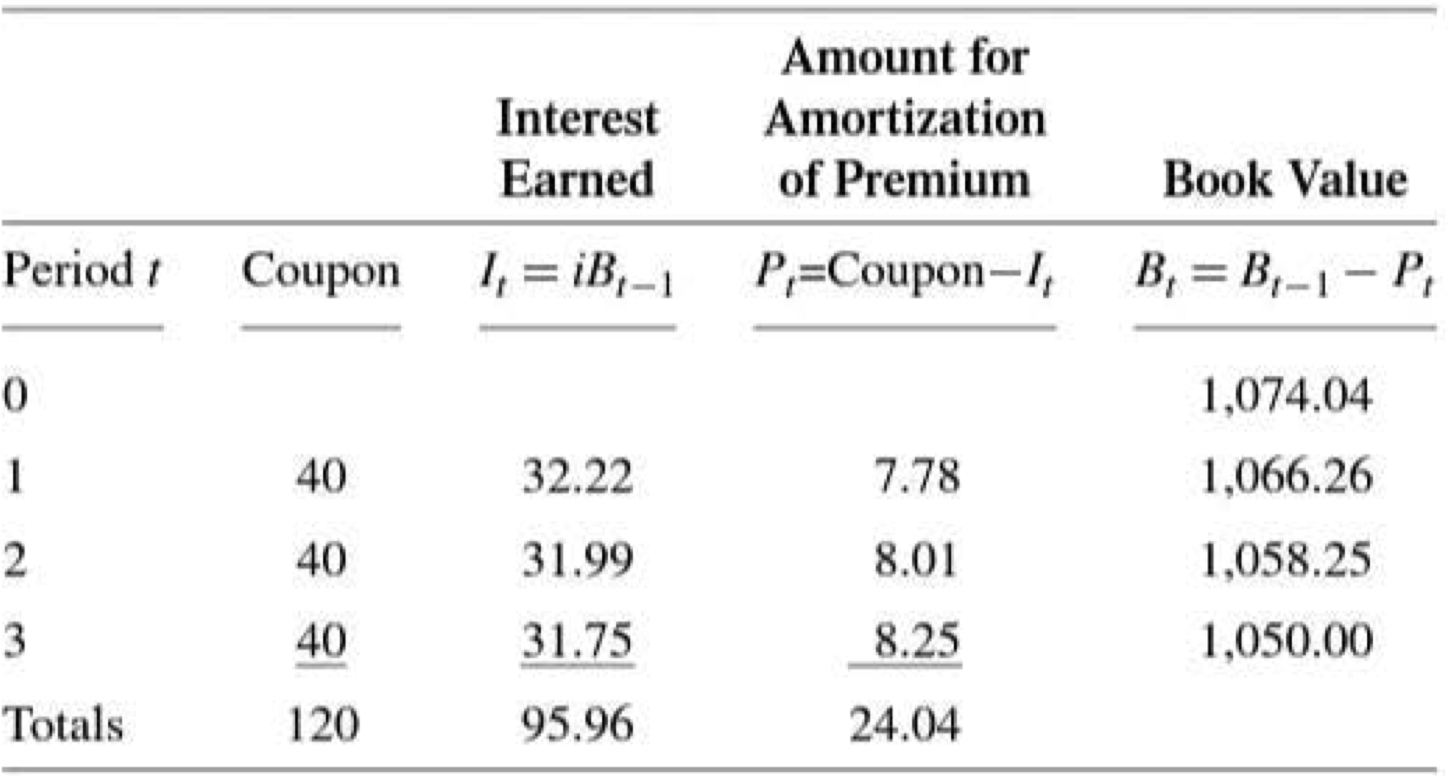
\includegraphics[scale=0.4]{img/amortization-schedule-bonds.png}
	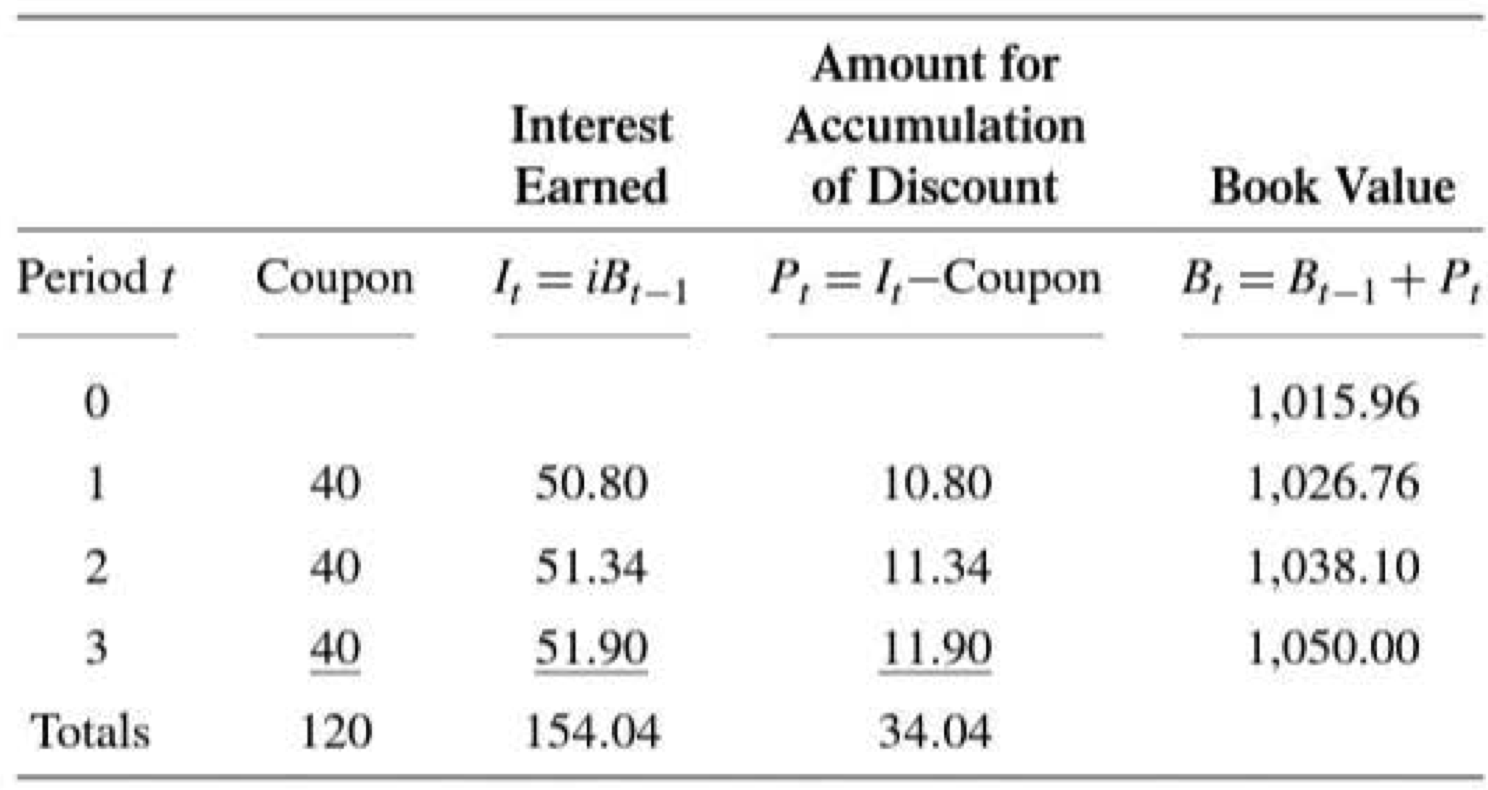
\includegraphics[scale=0.4]{img/amortization-schedule-bonds-discount.png}
\end{center}

\paragraph*{Note}	The amortization worksheet on the calculator can calculate values for us using the TVM values.
\end{CHPT_SUMM_AUTO}

\begin{CHPT_SUMM_AUTO}[label = {L.-7d}]{7d. Price Between Coupon Dates}
\paragraph*{2 types of prices between coupon dates}
\begin{enumerate}[leftmargin = *]
	\item	The price actually paid for the bond on the date of purchase (a.k.a. settlement date).
		\begin{itemize}[leftmargin = *]
		\item	Many names: "full price", "dirty price", "flat price", "price-plus-accrued".
		\item	$B_{t + k} = B_{t}(1 + i)^{k}, 0 \le k \le 1$.
		\item	This is the money that actually changes hands when the bond is sold.
		\end{itemize}
	\item	The price quoted for the bond in the financial press.
		\begin{itemize}[leftmargin = *]
		\item	Many names: "clean price", "market price", "price".
		\item	$B_{t + k} - kFr = B_{t}(1 + i)^{k} -kFr, 0 \le k \le 1$.
		\item	The practice is to quote this price which \textit{excludes the value of the coupon} which has \textit{accrued} by the date of purchase.
		\item	The \textit{accrued coupon} is commonly called the \textbf{\textit{accrued interest}}.
		\end{itemize}
\end{enumerate}

\

In practice, the price excluding accrued interest is quoted because the full price has a saw-toothed progression:
\begin{center}
	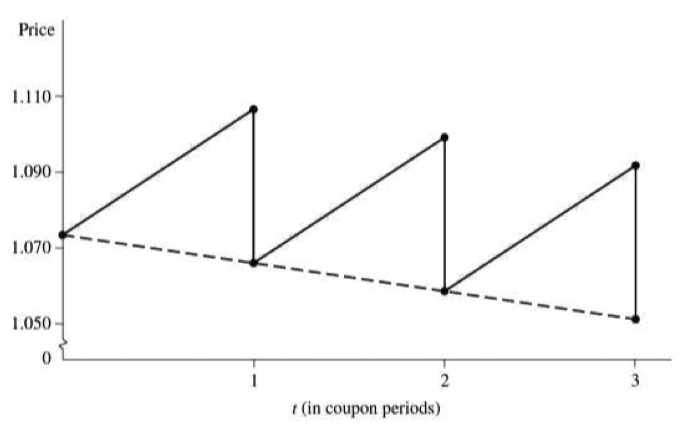
\includegraphics[scale=0.4]{img/BONDS-MRKTPRICE.png}
\end{center}

\tcbline

There are 2 methods of counting the days for the fraction $k = \frac{\text{days between last coupon and purchase date}}{\text{days between next coupon and purchase date}}$:
\begin{enumerate}[leftmargin = *]
	\item	The "actual/actual" method.
		\begin{itemize}[leftmargin = *]
		\item	This method is used for government bonds.
		\item	The actual number of days is used for both the numerator and denominator of $k$.
		\end{itemize}
	\item	The "30/360" method.
		\begin{itemize}[leftmargin = *]
		\item	This method is used for corporate and municipal bonds.
		\item	Each month is considered to have 30 days and a year assumed to have 360 to calculate $k$.
		\end{itemize}
\end{enumerate}
\end{CHPT_SUMM_AUTO}

\begin{CHPT_SUMM_AUTO}[label = {L.-7e}]{7e. Determination of Yield Rates}
It is likely we'll have to calculate a yield rate from the price of a bond and the remainder of the information. This cannot be done by hand and must be calculated with the financial calculator. \\
However, there is an approximation, \hl{which is not on the syllabus}, to approximate the yield rate---the \textbf{Bond Salesman's Method}.

\begin{align*}
	\text{Total interest}	
	&=	nCg + C - P	\\
	\text{\shortstack{Average interest\\ per period}}
	&=	\frac{nCg + C - P}{n}	\\
	\text{Average investment}
	&=	\frac{P + C}{2}	\\
	\text{\shortstack{Approximate yield\\ rate per period $i$}}
	&=	\frac{nCg + C - P}{\frac{n}{2}(P + C)}
\end{align*}
\end{CHPT_SUMM_AUTO}

\begin{CHPT_SUMM_AUTO}[label = {L.-7f}]{7f. Callable Bonds}
\paragraph*{Callable bonds}
\begin{itemize}[leftmargin = *]
	\item	The borrower (issuer) can redeem (a.k.a. call back or buy back) the bond prior to maturity.
	\item	There is generally a \textbf{call date} prior to which the issuer cannot call back the bond.
	\item	The \textbf{call price} is the redemption price the issuer must pay the lender if the bond is called.\\
			This price may differ from the regular redemption price $C$.
\end{itemize}

\paragraph*{Context}
\begin{itemize}[leftmargin = *]
	\item	Calling back the bond is advantageous for the issuer in case there is a decline in interest rates after issue---they could issue new bonds with lower coupons.
	\item	The difficulty with callable bonds for the investor is:
			\begin{itemize}[leftmargin = *]
			\item	The uncertainty of the term.
			\item	The difficulty in determining the yield rate relative to the selling price---if there is a decrease in the interest rate, the investor has to invest the redemption value for a lower return.
			\end{itemize}
\end{itemize}

\tcbline

Thus, to price these bonds we have to find the worst possible date of redemption at which we ensure a minimal return.
\begin{itemize}
	\item	For a bond selling at a \textbf{P}remium, the \textbf{E}arliest redemption date is the \textbf{W}orst one (\textbf{PEW} to remember).
	\item	For a bond selling at a discount, the latest redemption date is the worst one.
\end{itemize}
\end{CHPT_SUMM_AUTO}

